\subsection{Pruebas de firmware}

A nivel firmware, también se realizaron pruebas muy modularizadas para asegurarse el correcto funcionamiento de las interfaces con cada uno de los circuitos o módulos del sistema. \\ 

La comunicación con el módulo GPS se probó inicialmente por fuera del PCB, ya que los módulos (GPS y Nucleo) estaban disponibles antes de la fabricación de la placa. Para esto, se copiaron las conexiones esperadas utilizando cables externos para conectar las interfaces UART de la Nucleo con el módulo GPS. El módulo GPS viene con una configuración por defecto que trasmite a un \textit{baudrate} de 9600 una serie de mensajes una vez por segundo. Para verificar la comunicación entre los módulos, del lado del MCU se configuró la recepción por interrupción y se reenviaron todos los datos recibidos a la interfaz de debugging para poder ser inspeccionados. Se observó que efectivamente una vez por segundo se recibían todas las frases NMEA que indicaba la hoja de datos. A partir de esa estructura de datos identificada, se armó un \textit{parser} para poder extraer de la frase GPRMC los datos de estado de la comunicación GPS, la ubicación (latitud, longitud) y la velocidad informada. Estos datos también fueron enviados por la interfaz de debugging para luego verificar si estaban correctos. El módulo GPS puede perder la conexión con los satélites por lo que deja de informar todos los datos así que se probó el estado de conexión correcto y la pérdida de conexión desconectando la antena del sistema. \\ 

Con el módulo ESP32 también se realizaron las primeras pruebas de comunicación de manera externa. El ESP32 cuenta con una interfaz serie accesible mediante USB por lo que se configuró para retransmitir todo lo recibido por el MCU a través de esta interfaz y también retransmitir lo recibido por USB al MCU. La misma configuración se realizó en el MCU. Por lo tanto, al enviar un mensaje desde la PC al MCU, se recibía por la comunicación con el ESP32 el mismo mensaje y al enviar desde la PC un mensaje al ESP32, se recibía el mismo mensaje por la interfaz con el MCU. De esta manera, se verificó que la comunicación entre los módulos era correcta y se estaban procesando correctamente los mensajes trasmitidos y recibidos. Luego, se configuró el ESP32 para conectarse a una red Wi-Fi y al servidor MQTT, por lo que se modificó el firmware para retransmitir ya no a través de la interfaz USB, sino a través del servidor MQTT. Desde la PC, se configuró el broker MQTT en shifr.io y se conectó como cliente utilizando la librería Paho \cite{paho} de Python para interactuar con el servidor. Con esta extensión, se pudo repetir la prueba de comunicación entre el MCU principal, el ESP32 y el servidor MQTT, ya que los mensajes llegaban correctamente de punta a punta en ambos sentidos. Las conexiones utilizadas para esta último escenario se pueden visualizar en la figura \ref{fig:mqtt_testbench} 


\begin{figure}[H]
    \centering
    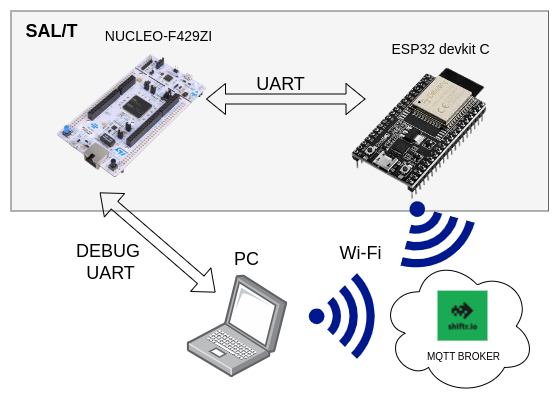
\includegraphics[width = 0.7\linewidth]{img/mqtt_testbench.png}
    \caption{Conexiones para prueba de comunicación con ESP32 y servidor MQTT}
    \label{fig:mqtt_testbench}
\end{figure}

Para el código del ESP32, también se realizó la prueba de configurarle la conexión a 2 redes Wi-Fi y cuando no se pueda conectar a una, intentar la conexión con la otra de manera sistemática. Se levantaron 2 redes Wi-Fi y se probó que al desconectar una, se conecta con la otra (envía un log al servidor MQTT cuando se conecta a una nueva red) y al desconectarse ambas se queda monitoreando qué red se levanta primero para establecer una conexión lo antes posible. \\ 

Para la comunicación con la tarjeta SD, también se logró realizar algunas pruebas anticipadas a tener la placa lista. Para esto, se utilizó un módulo para tarjetas microSD \cite{modulo_sd} reutilizado de otro proyecto que se puede observar en la figura \ref{fig:modulo_sd}. Este módulo, permite conectar solo las señales de SPI con cables externos a la placa Núcleo. Se realizó esta conexión y se probaron algunas funciones básicas de la comunicación como listar los archivos disponibles dentro de la unidad, escribir en un archivo y leer el contenido de un archivo. Con estas pruebas básicas y el desarrollo de las funciones para interactuar, se verificó el funcionamiento en la comunicación por SPI con la tarjeta SD. Una vez recibidas las placas, se realizaron las mismas pruebas, pero utilizando el zócalo para la tarjeta microSD soldado a la placa principal junto a las resistencias diseñadas para las lineas de comunicación. 

\begin{figure}[H]
    \centering
    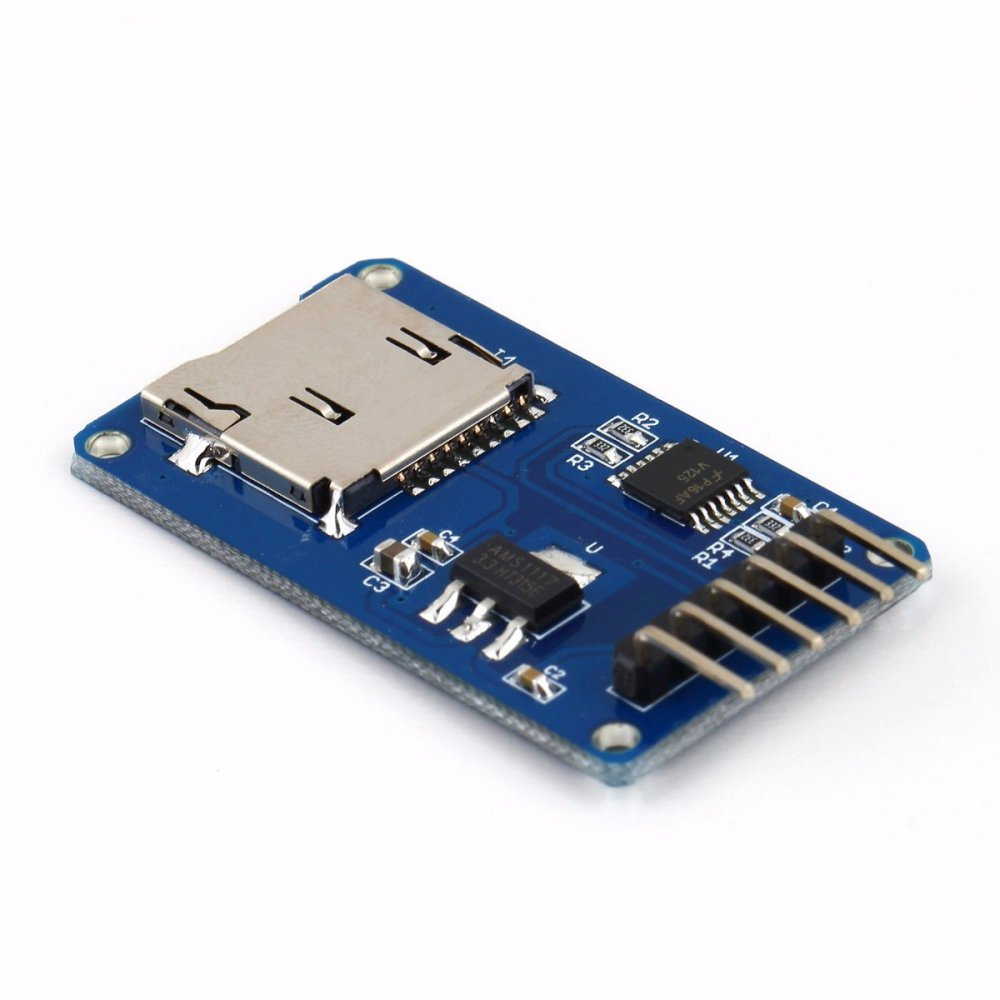
\includegraphics[width = 0.4\linewidth]{img/modulo_sd.jpg}
    \caption{Módulo SD para pruebas de comunicación}
    \label{fig:modulo_sd}
\end{figure}

Para la comunicación con las fuentes de velocidades externas, se utilizó un Arduino Uno y módulos conversor UART a RS485 para poder conectar con el SAL/T. En estas comunicaciones, se configuró el Arduino para transmitir de manera continua distintas velocidades en el formato esperado de cada uno de los sistemas que simula. Para el generado de impulsos ópticos, se envía el dato numérico de la velocidad directo, y para la señal proveniente del Hasler Teloc 1500 se envía una trama de 31 bytes con el dato de velocidad en los bytes 7 y 8. Del lado del SAL/T, se conectan las interfaces RS485 con el pin de selección de dirección de la comunicación en modo recepción y se procesan los mensajes recibidos y se envían por interfaz de debugging para visualizarlos desde una PC. En ambas comunicaciones se logró obtener el dato de la velocidad transmitido y asociado a la interfaz del cual proviene cada dato. \\ 

Por último, se realizaron varias pruebas de comunicación y configuración con el controlador LED. Una vez con las placas armadas, ya que el empaquetado del chip no permitía una conexión con cables externos, se realizaron algunas pruebas utilizando el protocolo I2C. Utilizando la hoja de datos como referencia, se escribieron algunos registros para validar la comunicación y el funcionamiento deseado del controlador LED y de los LEDs conectados. Primero se habilitaron todos los dígitos que puede controlar el chip y se fueron encendiendo uno a uno los segmentos y LEDs conectados en un orden específico. Esto permitió verificar el mapeo entre las variables que representan un estado y la posición dentro de un registro del controlador. Una vez validado el mapeo, se armaron alguna funciones que permiten escribir los registros del controlador LED solamente utilizando el estado de los LEDs individuales y el número a mostrar para los dígitos 7 segmentos. De esta manera, se hicieron varias pruebas de escribir todas las cifras en el display y de encender y apagar todos los estados visualizables para verlo reflejado en los LEDs de la placa secundaria. También se probó la escritura de registros de configuración como el ajuste del brillo o la deshabilitación de alguno de los dígitos controlados o el reset por software que permite el controlador. 